\documentclass{beamer}
\usepackage[italian]{babel}
\usepackage[utf8]{inputenc}
\usepackage[T1]{fontenc}

% Personal commands
\newcommand{\code}[1]{\mbox{\texttt{#1}}}
\newcommand{\command}[1]{\mbox{\texttt{#1}}}
\newcommand{\file}[1]{\mbox{\texttt{#1}}}

% Beamer options
\beamertemplatenavigationsymbolsempty
\setbeamertemplate{bibliography item}{}
\setbeamertemplate{caption}{\insertcaption}
\setbeamertemplate{footline}[frame number]

\title{Network Security}
\author[leot]{Leonardo Taccari \\ {\footnotesize \texttt{<s1069964@studenti.univpm.it>}}}
\date{}

\begin{document}

% Title of the presentation
\begin{frame}
\maketitle
\end{frame}

% Outline
\begin{frame}{Sommario}
\tableofcontents
\end{frame}

\section{Modello ISO/OSI e TCP/IP}
\subsection{Modello ISO/OSI}
\begin{frame}{\insertsection}
\begin{figure}
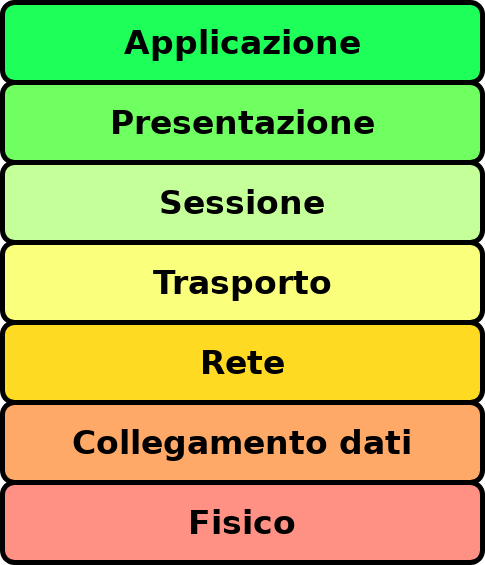
\includegraphics[width=0.35\textwidth]{imgs/01-iso-osi.drawio.png}
\caption{Modello ISO/OSI}
\end{figure}
\end{frame}

\subsection{Strati del modello ISO/OSI}
\subsubsection*{Fisico}
\begin{frame}{\insertsection}{\insertsubsection}
\begin{columns}
\column{0.2\textwidth}
\begin{figure}
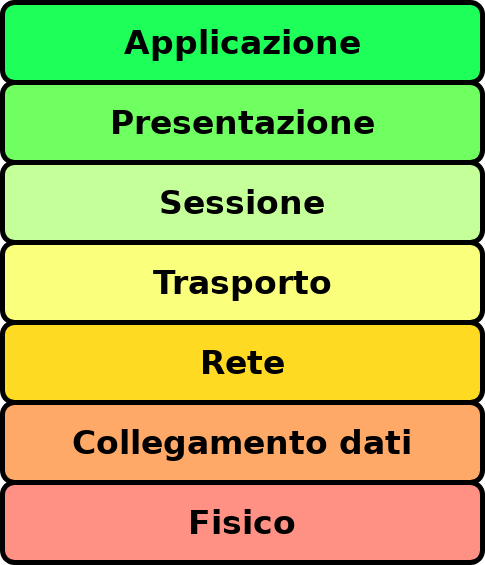
\includegraphics[width=0.95\textwidth]{imgs/01-iso-osi.drawio.png}
\end{figure}
\column{0.75\textwidth}
\begin{block}{\insertsubsubsection}
Trasmissione di un flusso di bit attraverso un collegamento fisico tra nodi.
\end{block}
\end{columns}
\end{frame}

\subsubsection*{Collegamento dati}
\begin{frame}{\insertsection}{\insertsubsection}
\begin{columns}
\column{0.2\textwidth}
\begin{figure}
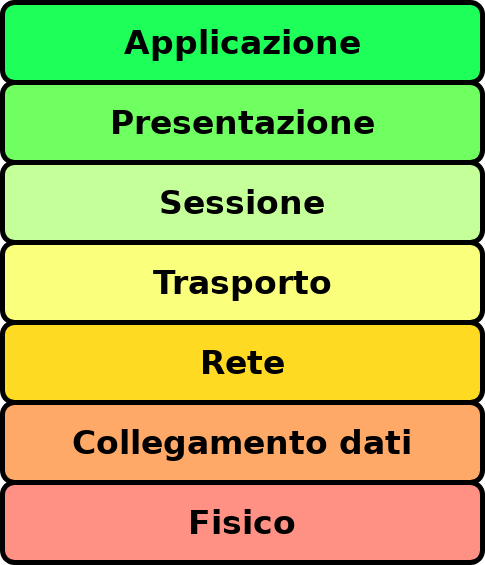
\includegraphics[width=0.95\textwidth]{imgs/01-iso-osi.drawio.png}
\end{figure}
\column{0.75\textwidth}
\begin{block}{\insertsubsubsection}
Trasmissione affidabile di frame di dati (insieme di bit) tra due nodi connessi a livello fisico.
\end{block}
\end{columns}
\end{frame}

\subsubsection*{Rete}
\begin{frame}{\insertsection}{\insertsubsection}
\begin{columns}
\column{0.2\textwidth}
\begin{figure}
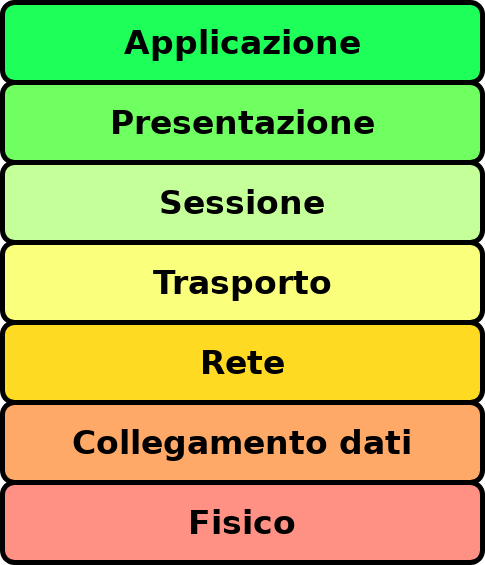
\includegraphics[width=0.95\textwidth]{imgs/01-iso-osi.drawio.png}
\end{figure}
\column{0.75\textwidth}
\begin{block}{\insertsubsubsection}
Trasmissione dei pacchetti dal nodo sorgente al nodo di destinazione
indipendentemente dalle tecnologie di trasmissione.
\end{block}
\end{columns}
\end{frame}

\subsubsection*{Trasporto}
\begin{frame}{\insertsection}{\insertsubsection}
\begin{columns}
\column{0.2\textwidth}
\begin{figure}
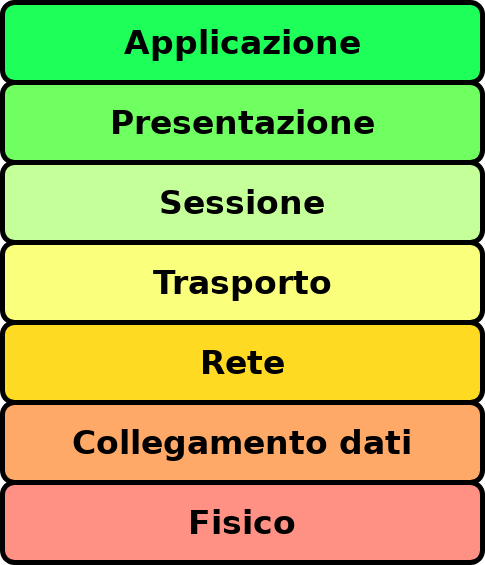
\includegraphics[width=0.95\textwidth]{imgs/01-iso-osi.drawio.png}
\end{figure}
\column{0.75\textwidth}
\begin{block}{\insertsubsubsection}
Trasmissione dei dati trasparente ed affidabile tra host.
\end{block}
\end{columns}
\end{frame}

\subsubsection*{Sessione}
\begin{frame}{\insertsection}{\insertsubsection}
\begin{columns}
\column{0.2\textwidth}
\begin{figure}
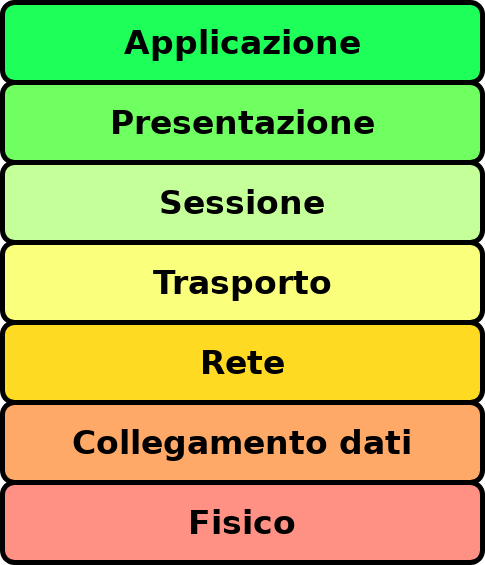
\includegraphics[width=0.95\textwidth]{imgs/01-iso-osi.drawio.png}
\end{figure}
\column{0.75\textwidth}
\begin{block}{\insertsubsubsection}
Controllare la comunicazione tra applicazioni instaurando, mantenendo e
chiudendo sessioni.
\end{block}
\end{columns}
\end{frame}

\subsubsection*{Presentazione}
\begin{frame}{\insertsection}{\insertsubsection}
\begin{columns}
\column{0.2\textwidth}
\begin{figure}
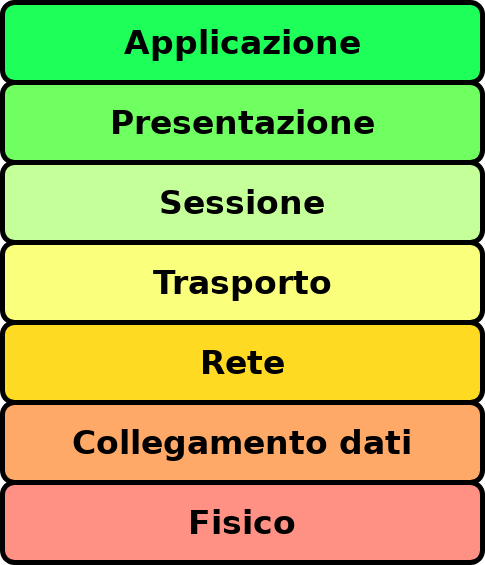
\includegraphics[width=0.95\textwidth]{imgs/01-iso-osi.drawio.png}
\end{figure}
\column{0.75\textwidth}
\begin{block}{\insertsubsubsection}
Trasformare i dati forniti formattandoli secondo un formato standard
((de)codifica, (de)compressione, (de)cifratura).
\end{block}
\end{columns}
\end{frame}

\subsubsection*{Applicazione}
\begin{frame}{\insertsection}{\insertsubsection}
\begin{columns}
\column{0.2\textwidth}
\begin{figure}
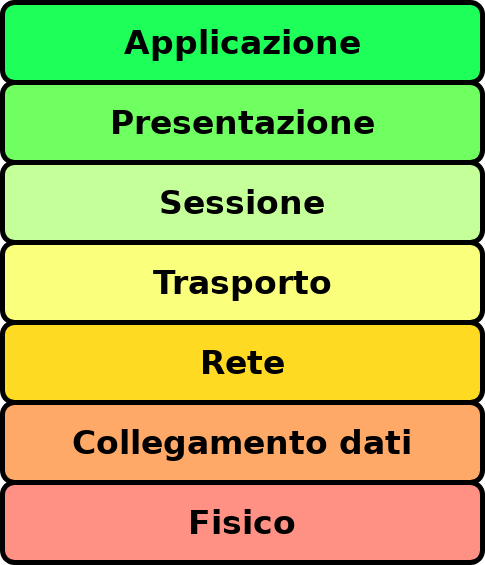
\includegraphics[width=0.95\textwidth]{imgs/01-iso-osi.drawio.png}
\end{figure}
\column{0.75\textwidth}
\begin{block}{\insertsubsubsection}
Fornire il servizio all'utente.
\end{block}
\end{columns}
\end{frame}

\subsection*{Analogia invio di una lettera ed ISO/OSI}
\begin{frame}{\insertsection}{\insertsubsection}
\begin{figure}
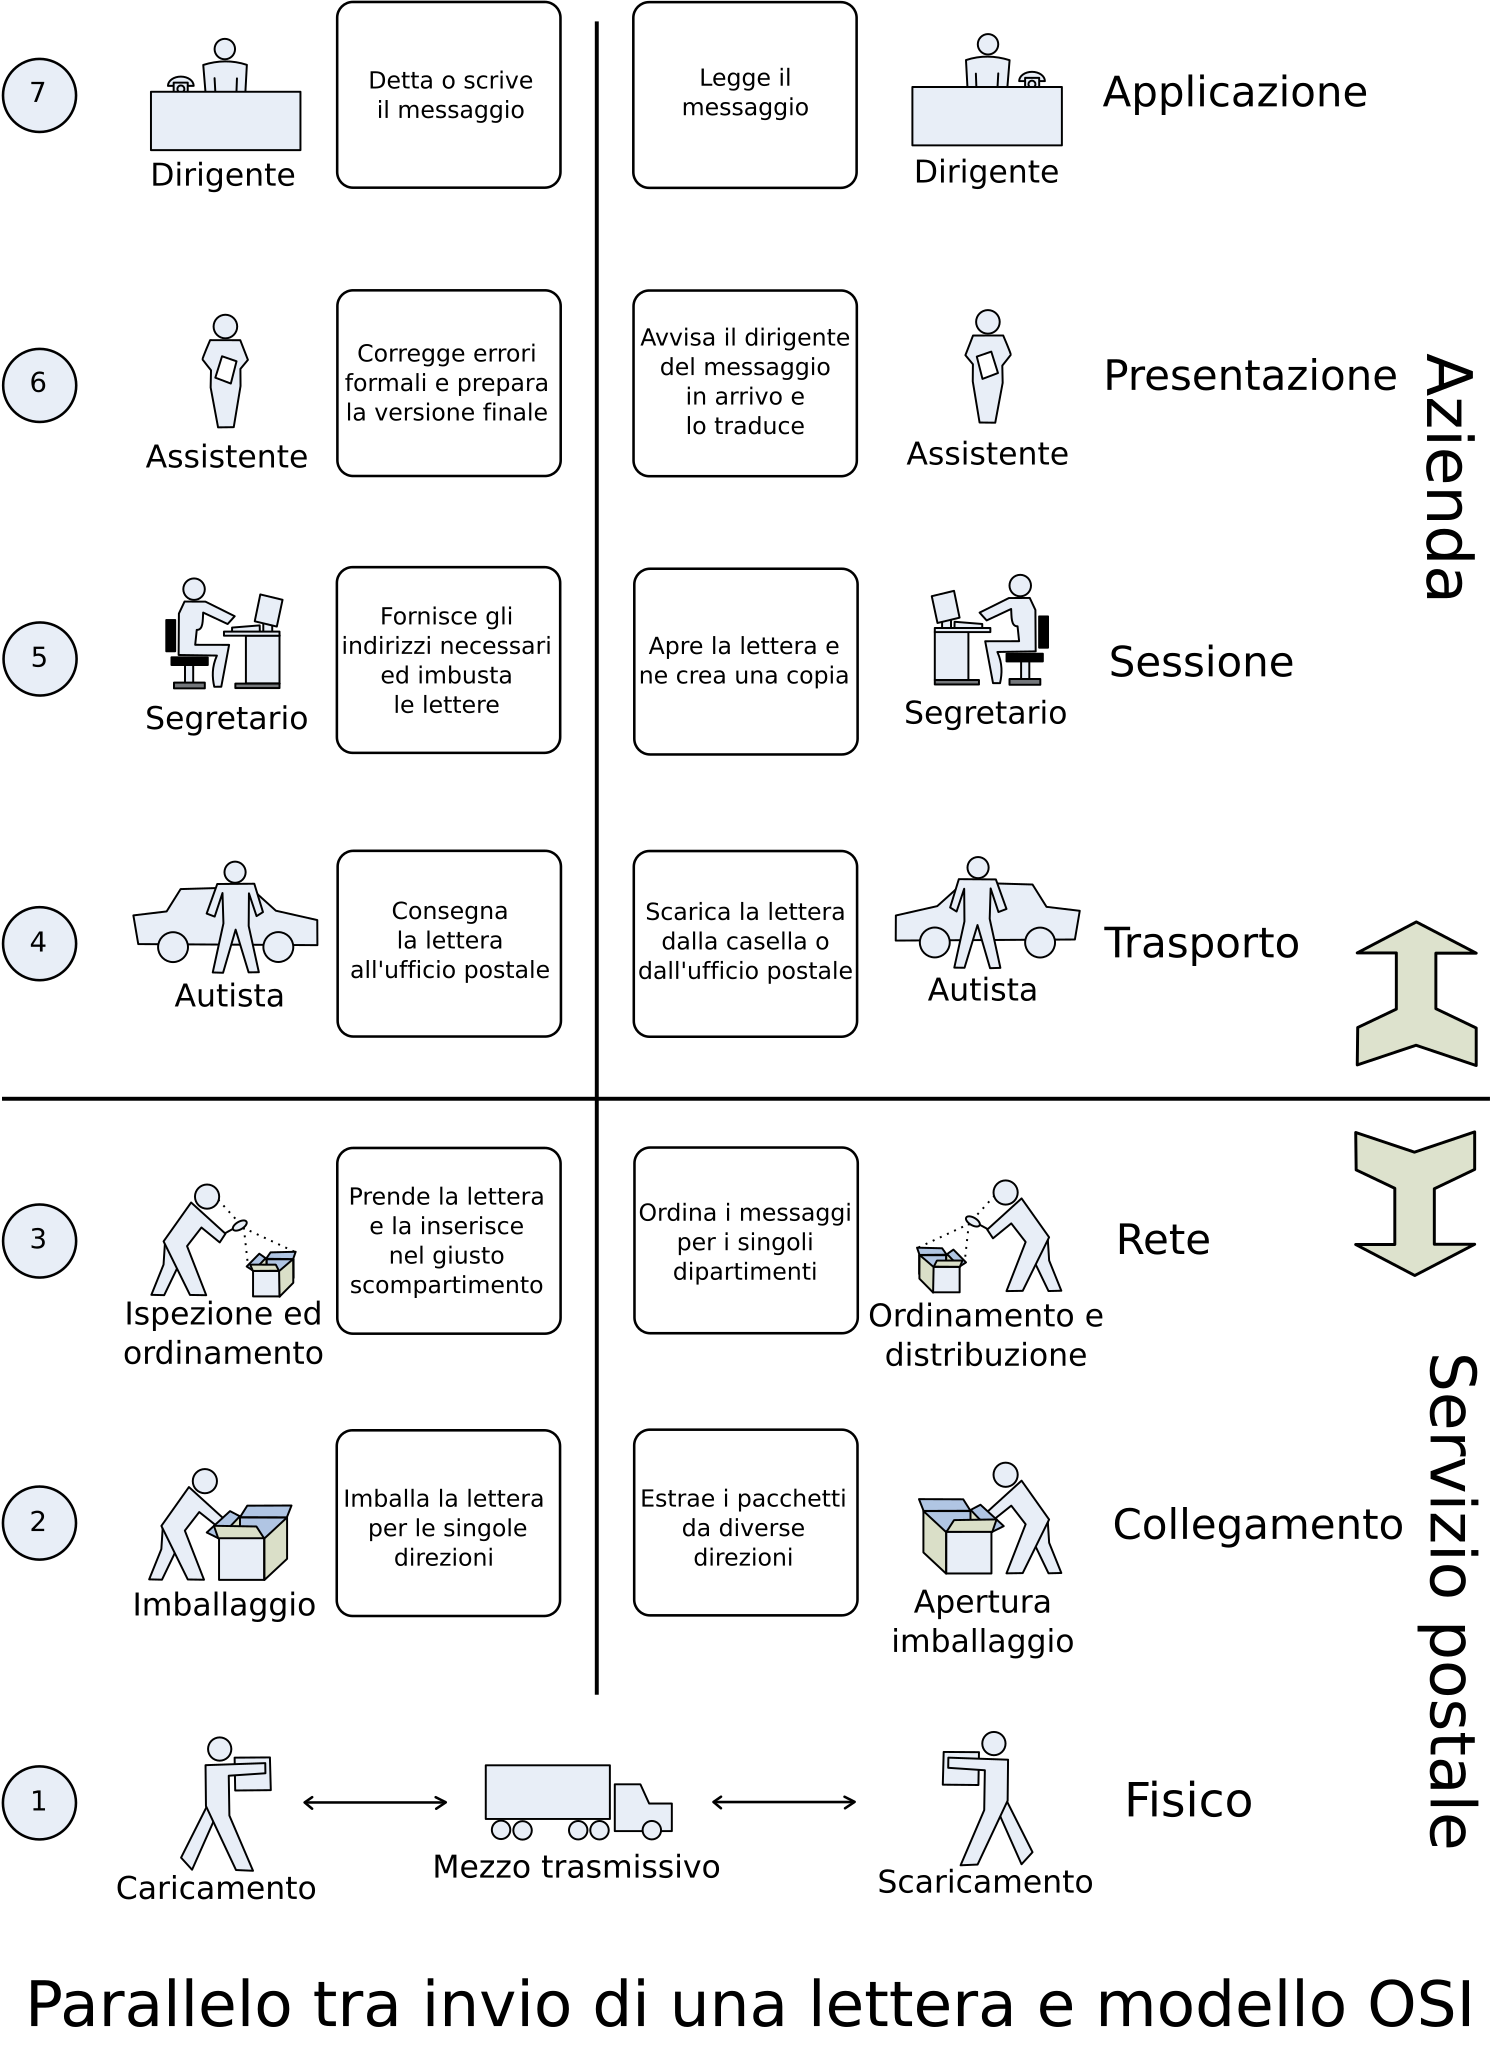
\includegraphics[width=0.40\textwidth]{imgs/lettera-e-iso-osi.png}
\caption{Dalla pagina \href{https://it.wikipedia.org/wiki/Modello\_OSI}{Modello
OSI} di Wikipedia, l'enciclopedia libera}
\end{figure}
\end{frame}

\subsection*{Protocols Data Unit (PDU)}
\begin{frame}{\insertsection}{\insertsubsection}
\begin{figure}
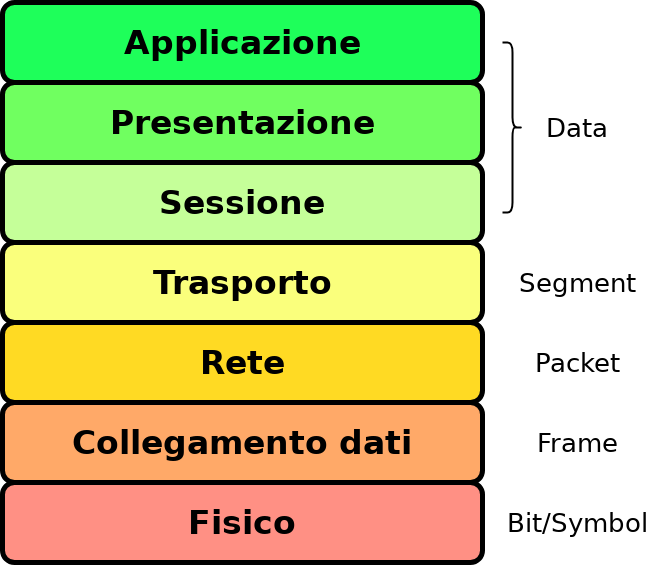
\includegraphics[width=0.35\textwidth]{imgs/02-iso-osi-pdu.drawio.png}
\caption{Protocols Data Unit (PDU)}
\end{figure}
\end{frame}

\subsection{TCP/IP}
\begin{frame}{\insertsection}{\insertsubsection}
\begin{figure}
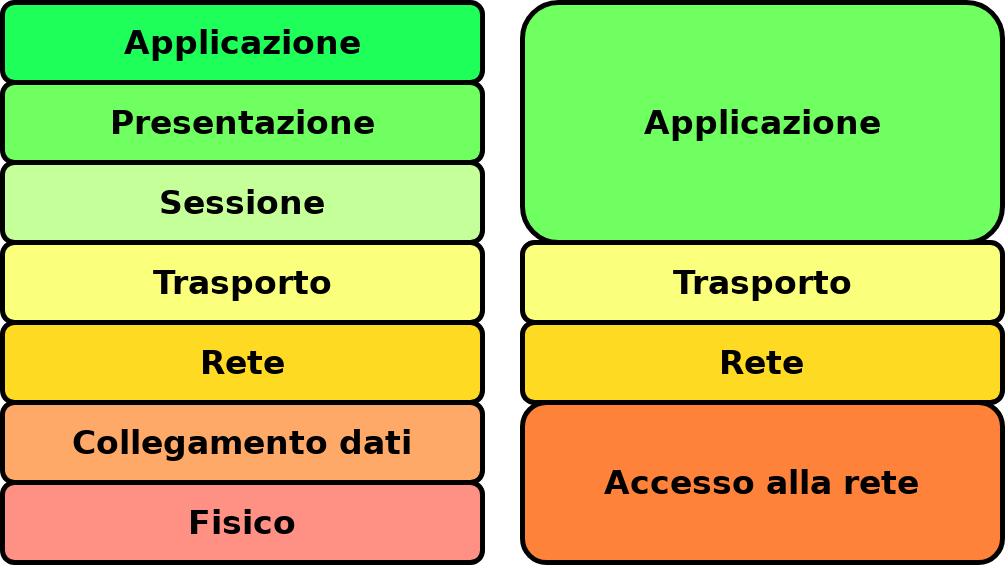
\includegraphics[width=0.60\textwidth]{imgs/03-iso-osi-tcp-ip.drawio.png}
\caption{Modello ISO/OSI e TCP/IP}
\end{figure}
\end{frame}


\subsection*{TCP/IP e Protocols Data Unit (PDU)}
\begin{frame}{\insertsection}{\insertsubsection}
\begin{figure}
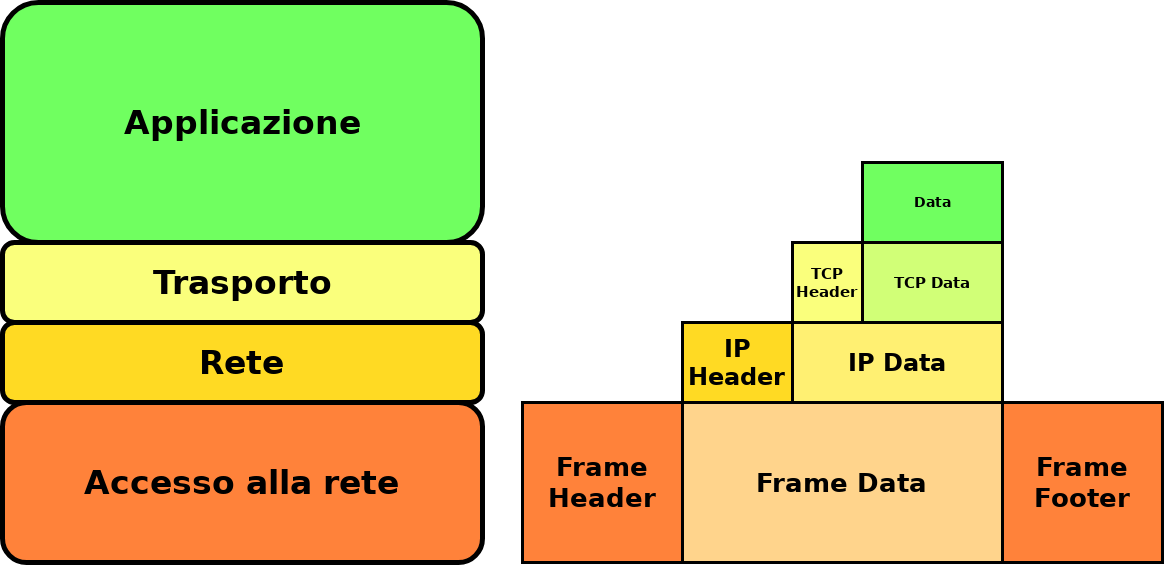
\includegraphics[width=0.60\textwidth]{imgs/04-tcp-pdu.drawio.png}
\caption{TCP/IP e Protocols Data Unit (PDU)}
\end{figure}
\end{frame}

\subsection*{TCP 3-way handshake}
\begin{frame}[allowframebreaks]{\insertsection}{\insertsubsection}
\begin{figure}
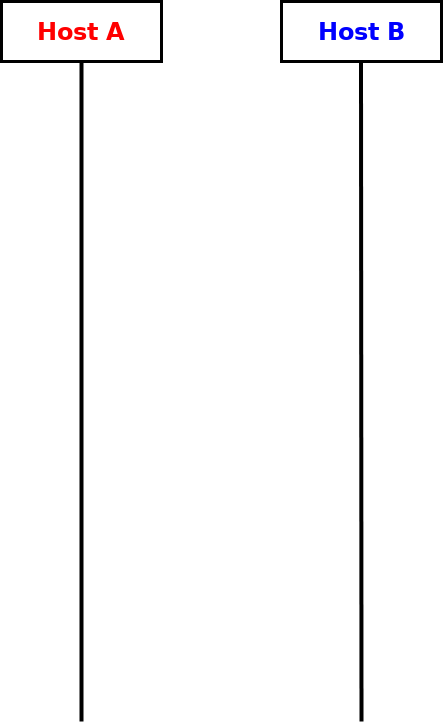
\includegraphics[width=0.37\textwidth]{imgs/tcp-3-way-handshake-00.drawio.png}
\end{figure}
\framebreak
\begin{figure}
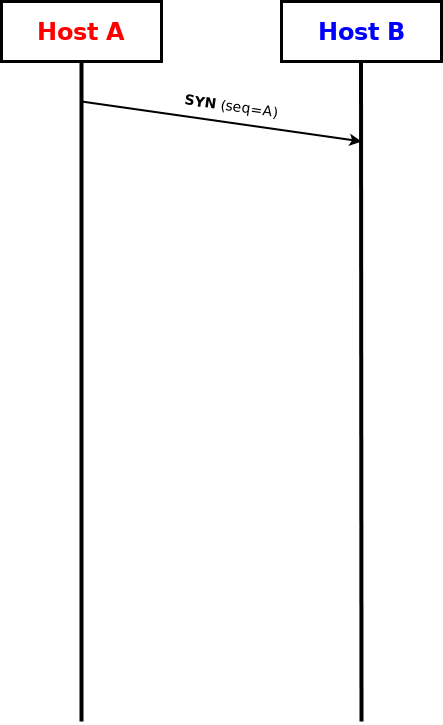
\includegraphics[width=0.37\textwidth]{imgs/tcp-3-way-handshake-01.drawio.png}
\end{figure}
\framebreak
\begin{figure}
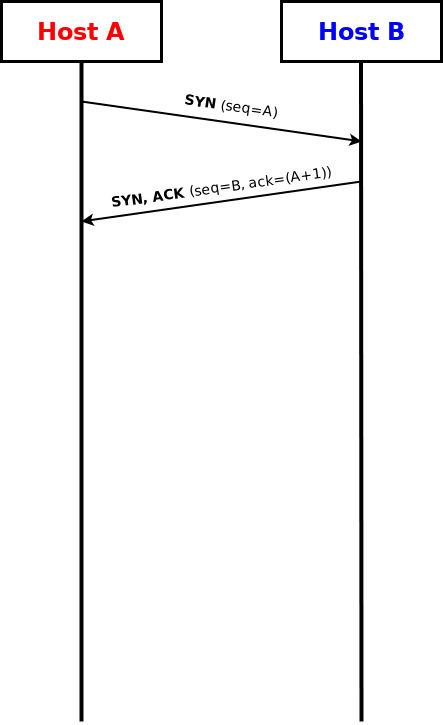
\includegraphics[width=0.37\textwidth]{imgs/tcp-3-way-handshake-02.drawio.png}
\end{figure}
\framebreak
\begin{figure}
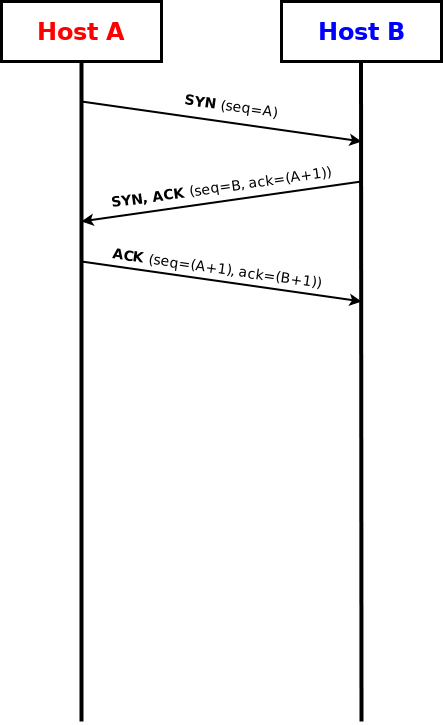
\includegraphics[width=0.37\textwidth]{imgs/tcp-3-way-handshake-03.drawio.png}
\end{figure}
\framebreak
\begin{figure}
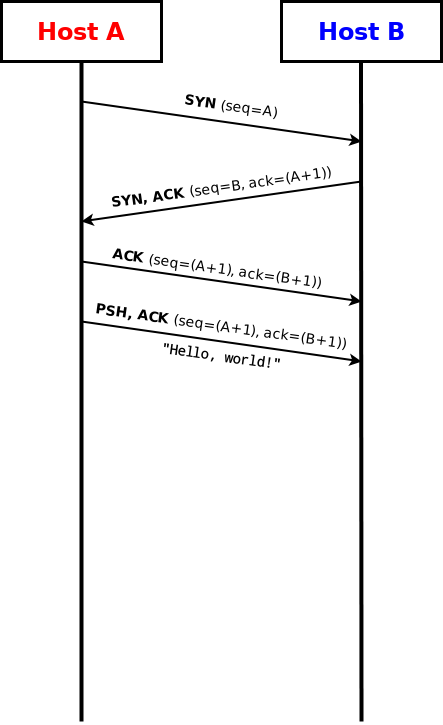
\includegraphics[width=0.37\textwidth]{imgs/tcp-3-way-handshake-04.drawio.png}
\end{figure}
\framebreak
\begin{figure}
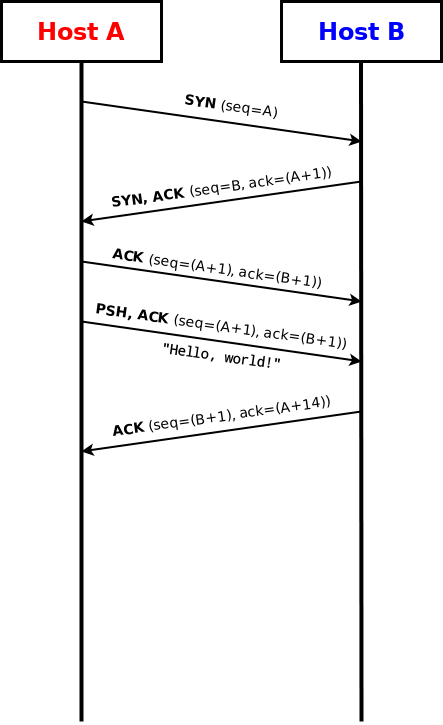
\includegraphics[width=0.37\textwidth]{imgs/tcp-3-way-handshake-05.drawio.png}
\end{figure}
\framebreak
\begin{figure}
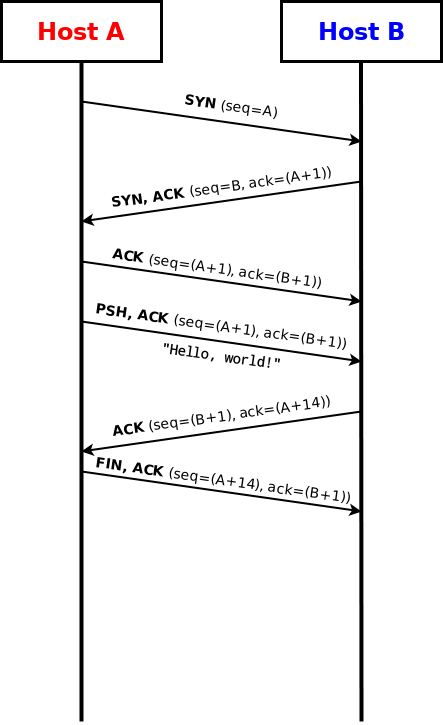
\includegraphics[width=0.37\textwidth]{imgs/tcp-3-way-handshake-06.drawio.png}
\end{figure}
\framebreak
\begin{figure}
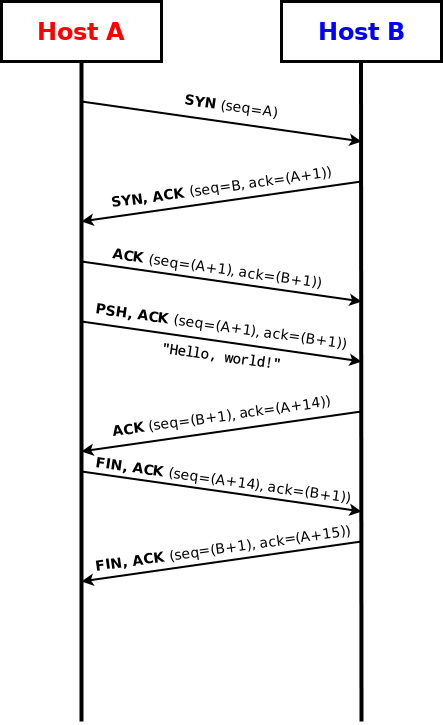
\includegraphics[width=0.37\textwidth]{imgs/tcp-3-way-handshake-07.drawio.png}
\end{figure}
\framebreak
\begin{figure}
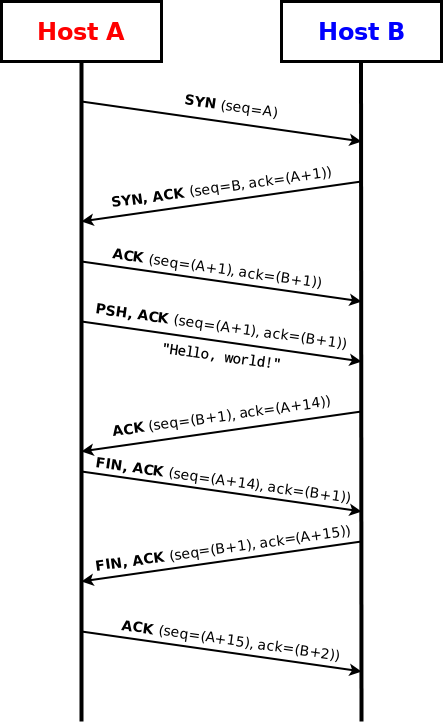
\includegraphics[width=0.37\textwidth]{imgs/tcp-3-way-handshake-08.drawio.png}
\end{figure}
\end{frame}

\section{Conclusioni}
\begin{frame}{\insertsection}
\begin{itemize}
\item Abbiamo visto il modello ISO/OSI e TCP/IP
\item Abbiamo visto come avviene il 3-way handshak nel protocollo TCP
\end{itemize}
\end{frame}

% FIXME: Use bibtex for that!
\section{Riferimenti}
\begin{frame}{\insertsection}
\begin{itemize}
\item \href{https://training.olicyber.it/training}{Materiale Didattico del Portale di allenamento delle Olimpiadi Italiane di Cybersicurezza} 
\end{itemize}
\end{frame}

\end{document}
